\documentclass[UTF8,12pt,a4paper]{ctexart}

\usepackage[left=2.5cm,right=2.5cm,top=2.5cm,bottom=2.5cm]{geometry}
\usepackage{amsmath}
\usepackage{graphicx}
\usepackage{booktabs}
\usepackage{xcolor}
\usepackage{listings}
\usepackage{float}
\usepackage{enumitem}
\usepackage{hyperref}
\usepackage{fancyhdr}

\hypersetup{
    colorlinks=true,
    linkcolor=blue,
    urlcolor=blue,
    citecolor=blue
}
% 页眉页脚
\pagestyle{fancy}
\fancyhf{}
\lhead{系统开发工具基础}
\rhead{第一周实验报告}
\cfoot{\thepage}

% 代码显示风格
\lstset{
    basicstyle=\ttfamily\small,
    breaklines=true,
    frame=single,
    columns=fullflexible,
    showstringspaces=false,
    numbers=left,
    numberstyle=\tiny\color{gray},
    keywordstyle=\color{blue},
    commentstyle=\color{green!50!black}
}

\title{系统开发工具基础\\第二周实验报告}
\author{姓名：林子钰 \\ 学号：25060012017  班级：计算机类1班}
\date{2026年8月31日}

\newpage
\usepackage{graphicx}
\usepackage{float}

\newcommand{\expimage}[3]{
    \begin{figure}[H]
        \centering
        \includegraphics[width=0.90\textwidth]{#1}
        \caption{#2}
        \label{#3}
    \end{figure}
}

\begin{document}

\maketitle
\tableofcontents
\newpage

\section{实验概述}

第二周实验主要围绕程序调试与性能分析展开，重点学习如何根据错误信息、调用栈和变量状态定位程序问题，并通过测试验证修复结果。

本周实验涉及语法错误、运行时错误和逻辑错误的排查，同时练习使用断点、单步执行、变量监视等调试方法。在归并排序实验中，需要重点检查循环条件和数组下标，例如将下标 j 错写为 i 可能导致排序结果错误。此外，还需要使用计时或性能分析工具查找程序运行瓶颈，对比优化前后的执行效率。

通过本周实验，我掌握了基本的程序调试和性能分析方法，理解了先保证程序正确、再进行性能优化的重要性，为后续深度学习和科研项目中的问题排查打下基础。



\section{实验环境}

\begin{table}[H]
    \centering
    \caption{实验环境}
    \label{tab:environment}
    \begin{tabular}{ll}
        \toprule
        项目 & 配置 \\
        \midrule
        操作系统 & Ubuntu 24.04.4 \\
        Shell & Bash \\
        Git 版本 & 2.34.1 \\
        LaTeX 环境 & pdfTeX 3.141592653-2.6-1.40.22 (TeX Live 2022/dev/Debian)
 \\
        编译引擎 & XeLaTeX \\
        编辑器 & GNU nano, version 6.2 \\
        \bottomrule
    \end{tabular}
\end{table}

\section{课堂实验}

\subsection{实验五：控制一个可清理的后台任务}

\subsubsection{实验目的}

1.掌握Shell前台任务与后台任务的基本概念。
2.掌握使用 Ctrl-Z 暂停前台进程、使用 bg 将任务放入后台运行的方法。
3.掌握使用 jobs 查看Shell作业、使用 jobs -p 获取进程号的方法。
4.理解Linux信号机制，能够使用 kill -TERM 向进程发送终止信号。
5.掌握Shell脚本中的 trap 命令，理解程序退出时执行清理操作的机制。

\subsubsection{关键过程}

\subsection{创建并运行Shell脚本}

首先创建实验脚本并赋予执行权限：

\begin{lstlisting}[language=bash]
touch worker.sh
chmod +x worker.sh
bash -n worker.sh
./worker.sh
\end{lstlisting}

其中，\texttt{touch}用于创建脚本文件，\texttt{chmod +x}为脚本添加执行权限，\texttt{bash -n}用于检查脚本语法，\texttt{./worker.sh}用于运行脚本。

\subsection{暂停前台任务并放入后台}

脚本运行后，按下\texttt{Ctrl-Z}暂停当前前台任务，然后执行以下命令：

\begin{lstlisting}[language=bash]
bg
jobs
\end{lstlisting}

\texttt{Ctrl-Z}会暂停前台进程，\texttt{bg}将暂停的任务放入后台继续运行，\texttt{jobs}用于查看当前Shell中的作业及其运行状态。

\subsection{获取进程号}

使用以下命令获取后台任务对应的进程号：

\begin{lstlisting}[language=bash]
jobs -p
pid=$(jobs -p | head -n 1)
printf "PID=%s\\n" "$pid"
\end{lstlisting}

\texttt{jobs -p}只输出作业对应的进程号。通过命令替换将进程号保存到变量\texttt{pid}中，便于后续发送信号。

\subsection{发送终止信号}

向后台进程发送\texttt{TERM}终止信号，并等待进程退出：

\begin{lstlisting}[language=bash]
kill -TERM "$pid"
wait "$pid"
\end{lstlisting}

\texttt{kill -TERM}用于向指定进程发送正常终止信号，\texttt{wait}用于等待后台进程结束，避免Shell过早执行后续命令。

\subsection{使用trap执行清理操作}

在脚本中使用\texttt{trap}捕获终止信号：

\begin{lstlisting}[language=bash]
trap 'echo CLEAN_EXIT >> cleanup.log; exit 0' TERM INT
\end{lstlisting}

当脚本接收到\texttt{TERM}或\texttt{INT}信号时，会将\texttt{CLEAN\_EXIT}写入\texttt{cleanup.log}，然后正常退出。该机制可以用于程序结束前释放资源、保存日志等清理操作。

\subsection{检查实验结果}

最后检查清理日志内容：

\begin{lstlisting}[language=bash]
cat cleanup.log
\end{lstlisting}

如果终端输出\texttt{CLEAN\_EXIT}，说明脚本成功捕获信号并执行了退出清理操作。

\subsubsection{实验结果}
\begin{figure}[htbp]
    \centering
    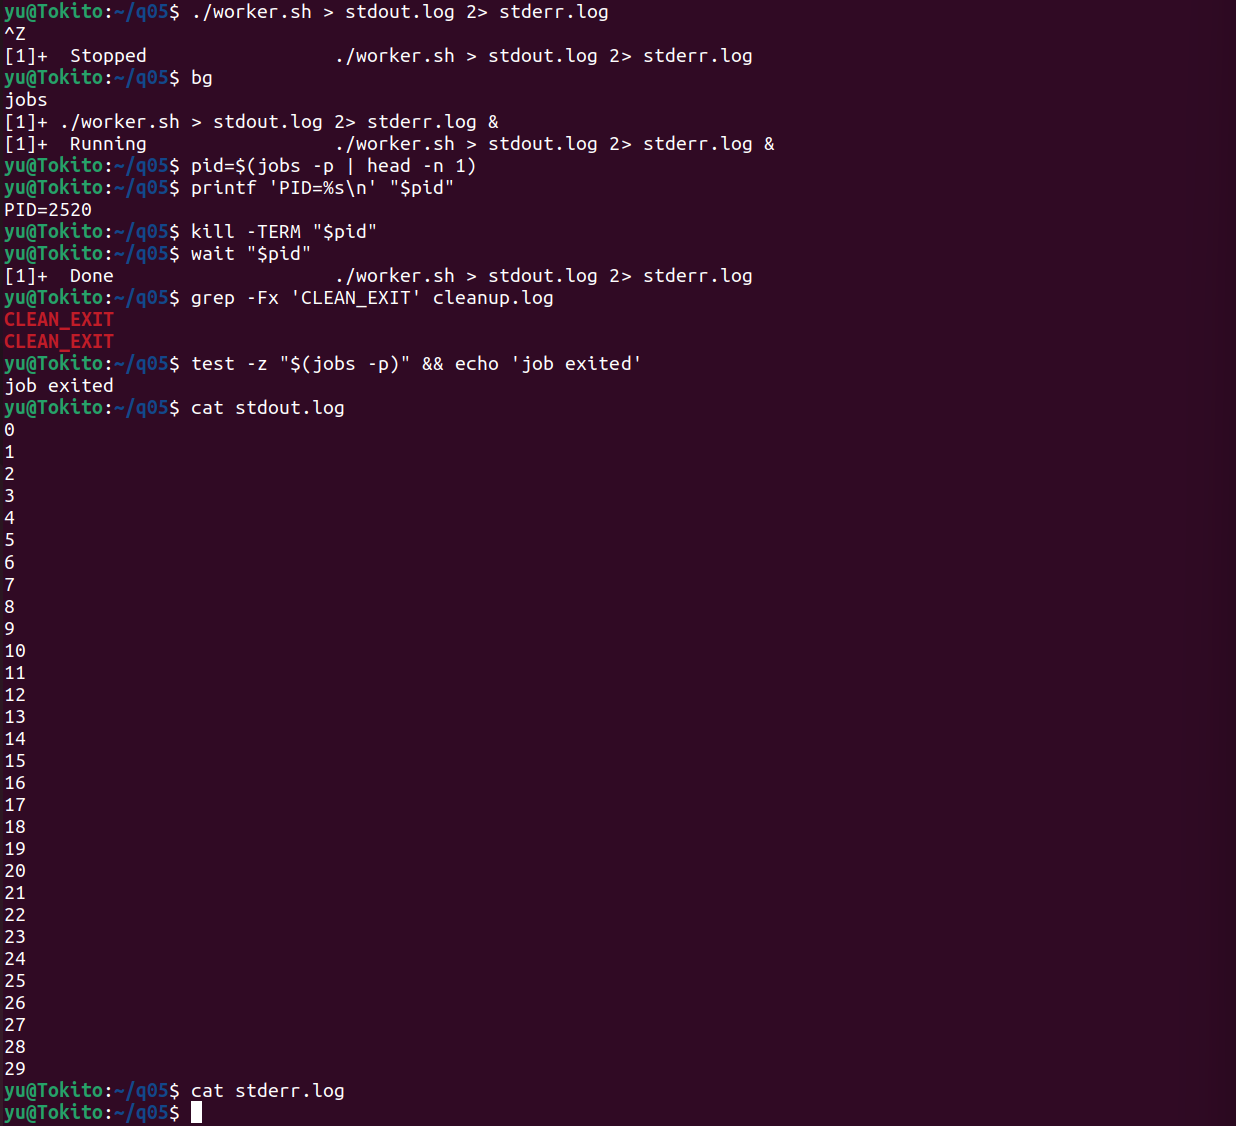
\includegraphics[width=0.95\textwidth]{../screenshots/q05/q05-result.png}
    \caption{Q05实验结果}
    \label{fig:q05-result}
\end{figure}
图~\ref{fig:q05-result}展示了Q05中Shell前后台任务切换、进程终止以及\texttt{trap}清理操作的关键运行结果。


实验结果表明，Shell脚本成功启动并在前台运行。按下\texttt{Ctrl-Z}后，前台任务被暂停，并显示为\texttt{Stopped}状态；执行\texttt{bg}命令后，该任务成功转入后台运行，\texttt{jobs}命令可以查看作业状态。

随后，通过\texttt{jobs -p}获取后台任务的进程号，例如\texttt{PID=2520}，并使用\texttt{kill -TERM}向该进程发送终止信号。\texttt{wait}命令等待后台任务结束，终端显示\texttt{Done}，说明进程已经正常退出。执行\texttt{grep}检查\texttt{cleanup.log}，成功输出\texttt{CLEAN\_EXIT}，表明\texttt{trap}命令已经捕获终止信号并完成清理操作。最后，使用\texttt{jobs -p}检查作业列表为空，并输出\texttt{job exited}。


\subsubsection{问题分析与体会}

本题需要重点理解Shell作业与进程之间的关系。\texttt{Ctrl-Z}只能暂停当前前台任务，任务暂停后还需要使用\texttt{bg}才能让它在后台继续运行；\texttt{jobs}用于查看当前Shell管理的作业，而\texttt{jobs -p}可以获取作业对应的进程号。

使用\texttt{kill -TERM}发送终止信号时，脚本不会简单地被强制结束，而是可以通过\texttt{trap}捕获信号，执行日志记录和资源清理等操作。因此，在程序退出前安排清理逻辑非常重要。实际操作中还应注意，\texttt{wait}的对象必须是有效的进程号，并且应在终止后台任务后检查\texttt{cleanup.log}和作业状态，从而确认信号处理和清理过程确实执行成功。





\subsection{实验六：使用 Ruff 和 pytest 完善 Python 项目}

\textbf{实验目的：}学习 Python 项目的基本组织方式，掌握函数编写、程序调用、单元测试、代码规范检查以及 Git 分阶段提交等开发工具的使用方法。

创建实验目录：

\begin{lstlisting}[language=bash]
mkdir q06
cd q06
\end{lstlisting}

创建 Python 工具函数文件 \texttt{math\_utils.py}：

\begin{lstlisting}[language=bash]
printf 'def calculate_total(price: float, count: int) -> float:\n    return price * count\n' > math_utils.py
\end{lstlisting}

该函数接收商品单价和数量两个参数，并返回商品总价。参数类型和返回值类型使用类型注解进行说明。

创建程序入口文件 \texttt{app.py}：

\begin{lstlisting}[language=bash]
printf 'from math_utils import calculate_total\n\nprint(calculate_total(12.5, 4))\n' > app.py
\end{lstlisting}

运行程序：

\begin{lstlisting}[language=bash]
python3 app.py
\end{lstlisting}

程序输出结果如下：

\begin{lstlisting}
50.0
\end{lstlisting}

这说明程序能够正确导入 \texttt{calculate\_total} 函数，并计算出单价为 $12.5$、数量为 $4$ 时的商品总价。

创建测试文件 \texttt{test\_math\_utils.py}：
\begin{lstlisting}[language=bash]
printf 'from math_utils import calculate_total\n\n\ndef test_calculate_total():\n    assert calculate_total(12.5, 4) == 50.0\n' > test_math_utils.py
\end{lstlisting}

运行 pytest 测试：

\begin{lstlisting}[language=bash]
python3 -m pytest -q
\end{lstlisting}

首次运行测试时，如果系统尚未安装 pytest，终端会提示：

\begin{lstlisting}
/usr/bin/python3: No module named pytest
\end{lstlisting}

此时更新软件源并安装 pytest：

\begin{lstlisting}[language=bash]
sudo apt update
sudo apt install -y python3-pytest
\end{lstlisting}

安装完成后再次运行测试：

\begin{lstlisting}[language=bash]
python3 -m pytest -q
\end{lstlisting}

测试结果如下：

\begin{lstlisting}
1 passed in ...s
\end{lstlisting}

测试结果显示共有一个测试用例通过，说明 \texttt{calculate\_total} 函数能够得到预期结果。
安装 Ruff 并进行代码质量检查：

\begin{lstlisting}[language=bash]
sudo snap install ruff
ruff --version
ruff check .
\end{lstlisting}

如果 Ruff 检测到代码格式或导入顺序问题，可以使用以下命令自动修复：

\begin{lstlisting}[language=bash]
ruff check . --fix
ruff check .
\end{lstlisting}

修复完成后，检查结果如下：

\begin{lstlisting}
All checks passed!
\end{lstlisting}

这表明当前项目中的 Python 文件已经通过 Ruff 的代码质量检查。

修改函数名称并检查项目：

\begin{lstlisting}[language=bash]
sed -i 's/total_price/calculate_total/g' math_utils.py app.py test_math_utils.py
python3 app.py
python3 -m pytest -q
ruff check .
\end{lstlisting}

运行结果如下：

\begin{lstlisting}
50.0
1 passed in ...s
All checks passed!
\end{lstlisting}

修改函数名称后，程序运行结果、单元测试结果和 Ruff 检查结果均正常。在修改过程中，如果终端提示语法错误，应根据错误提示检查对应文件，重点查看导入语句是否重复拼接、括号是否匹配以及缩进是否正确。

创建 Git 仓库并配置主分支：

\begin{lstlisting}[language=bash]
git init
git branch -M main
\end{lstlisting}

创建 `.gitignore` 文件，忽略 Python 运行过程中自动生成的缓存目录和字节码文件：

\begin{lstlisting}[language=bash]
printf '__pycache__/\n.pytest_cache/\n*.py[cod]\n' > .gitignore
\end{lstlisting}

查看当前文件状态：

\begin{lstlisting}[language=bash]
git status
\end{lstlisting}

进行第一次分阶段提交，提交 `.gitignore` 文件：

\begin{lstlisting}[language=bash]
git add .gitignore
git commit -m "chore: ignore Python cache files"
\end{lstlisting}

进行第二次提交，提交核心功能代码：

\begin{lstlisting}[language=bash]
git add math_utils.py
git commit -m "feat: add calculate_total utility"
\end{lstlisting}

进行第三次提交，提交程序入口和测试代码：

\begin{lstlisting}[language=bash]
git add app.py test_math_utils.py
git commit -m "test: add calculate_total usage and test"
\end{lstlisting}

本实验按照文件功能进行分阶段提交，没有将所有文件一次性提交。查看提交历史：

\begin{lstlisting}[language=bash]
git log --oneline --graph --all
\end{lstlisting}

提交历史示例如下：

\begin{lstlisting}
e665c9d (HEAD -> main) test: add calculate_total usage and test
6bca5b3 feat: add calculate_total utility
91367ac chore: ignore Python cache files
\end{lstlisting}

检查 Git 工作区状态：

\begin{lstlisting}[language=bash]
git status
\end{lstlisting}

如果所有文件均已提交，终端会显示：

\begin{lstlisting}
On branch main
nothing to commit, working tree clean
\end{lstlisting}

这说明当前 Git 工作区干净，没有未提交的修改。

配置并查看远程仓库：

\begin{lstlisting}[language=bash]
git remote add origin https://github.com/Tokito-git/sdt_week2-25060012017.git
git remote -v
\end{lstlisting}

远程仓库地址如下：

\begin{lstlisting}
https://github.com/Tokito-git/sdt_week2-25060012017.git
\end{lstlisting}

如果执行远程推送时出现连接被拒绝或网络超时，说明当前环境暂时无法连接 GitHub。此时本地代码编写、测试、代码规范检查和 Git 分阶段提交仍然已经完成；网络恢复后可以使用以下命令继续上传：

\begin{lstlisting}[language=bash]
git push -u origin main
\end{lstlisting}

\expimage{../screenshots/q06/q06-pro1-create_files.png}
{创建实验文件并检查 Python 代码}
{fig:q06-create-files}

\expimage{../screenshots/q06/q06-pro2-install_pytest.png}
{更新软件源并安装 pytest}
{fig:q06-install-pytest}

\expimage{../screenshots/q06/q06-pro3-install_configure_ruff.png}
{安装 Ruff 并修复代码格式问题}
{fig:q06-configure-ruff}

\expimage{../screenshots/q06/q06-pro4-rename_debug_code.png}
{修改函数名称并排查语法错误}
{fig:q06-rename-debug}

\expimage{../screenshots/q06/q06-pro5-create_commits.png}
{初始化 Git 仓库并完成分阶段提交}
{fig:q06-create-commits}

\expimage{../screenshots/q06/q06-result_1.png}
{代码检查、单元测试和程序运行结果}
{fig:q06-result-1}

\textbf{实验结果：}本实验完成了一个简单的 Python 计算项目，实现了 `calculate\_total` 函数，并通过程序调用验证其输出结果为 $50.0$。pytest 测试结果为 `1 passed`，Ruff 检查结果为 `All checks passed!`，说明当前代码能够正常运行并符合基本代码规范。

实验同时使用 Git 完成了三次分阶段提交，提交内容分别对应缓存文件忽略配置、核心功能函数以及程序入口和测试代码。最终 Git 工作区状态为 clean，满足实验对代码管理和提交记录的要求。

\textbf{实验体会：}通过本次实验，我认识到程序能够运行并不代表代码质量已经合格。pytest 可以验证功能是否正确，Ruff 可以发现代码规范问题，而 Git 分阶段提交则能够清晰记录开发过程。以后进行科研实验或深度学习项目开发时，测试、代码检查和版本管理都能够帮助快速定位问题，减少重复调试的时间。

\textbf{注意：}Python 项目中应将 `\_\_pycache\_\_`、`.pytest\_cache` 等自动生成目录写入 `.gitignore`，避免将无关缓存文件提交到仓库。代码修改后应依次运行程序、pytest 和 Ruff 检查，确认结果正确后再进行 Git 提交。实验必须分阶段提交，不能最后一次性提交全部文件，并应在实验报告中记录各次 commit 的作用。


\subsection{实验七：使用 pdb、pytest 和 Git 调试归并排序程序}

\textbf{实验目的：}学习使用 Python 调试器 pdb 定位程序错误，掌握归并排序算法的实现与修正方法，理解单元测试在验证程序正确性中的作用，并通过 Git 分阶段提交记录代码修改过程。

创建实验目录并进入 q07 目录：

\begin{lstlisting}[language=bash]
cd ~/sdt-week2/q07
\end{lstlisting}

查看并修改归并排序程序 \texttt{merge\_sort.py}。实验初始阶段，程序存在缩进错误、语法错误和归并过程中的下标错误。第一次运行时，终端报错如下：

\begin{lstlisting}
IndentationError: expected an indented block after function definition
SyntaxError: expected ':'
\end{lstlisting}

根据错误提示检查代码后，继续运行程序并进入 pdb 调试模式，观察归并过程中左右子数组和下标变量的变化情况：

\begin{lstlisting}[language=bash]
python3 merge_sort.py
\end{lstlisting}

在 pdb 中依次查看变量：

\begin{lstlisting}
p left
p right
p i
p j
p left[i]
p right[j]
\end{lstlisting}

调试过程中发现，归并操作里将右侧数组元素写成了 \texttt{right[i]}，正确写法应为 \texttt{right[j]}。这属于典型的循环下标错误，会导致归并结果异常。根据调试信息修正代码后，程序能够正常运行。

修正后的关键代码如下：

\begin{lstlisting}[language=python]
def merge(left, right):
    result = []
    i = 0
    j = 0
    while i < len(left) and j < len(right):
        if left[i] <= right[j]:
            result.append(left[i])
            i += 1
        else:
            result.append(right[j])
            j += 1
\end{lstlisting}

继续运行程序：

\begin{lstlisting}[language=bash]
python3 merge_sort.py
\end{lstlisting}

程序输出结果如下：

\begin{lstlisting}
[1, 1, 2, 3, 4, 5, 6, 9]
\end{lstlisting}

这说明归并排序程序已经能够正确输出排序结果。

创建并运行单元测试，使用 pytest 验证归并排序功能：

\begin{lstlisting}[language=bash]
python3 -m pytest -v
\end{lstlisting}

测试结果如下：

\begin{lstlisting}
collected 2 items

test_merge_sort.py::test_normal_input PASSED
test_merge_sort.py::test_duplicate_elements PASSED

2 passed in 0.06s
\end{lstlisting}

测试结果显示两个测试用例均通过，说明程序在普通输入和重复元素输入两种情况下都能正确运行。

创建 Git 仓库并进行分阶段提交：

\begin{lstlisting}[language=bash]
cd ~/sdt-week2
git init
git add q07/merge_sort.py
git commit -m "fix: correct merge sort index"
git add q07/test_merge_sort.py
git commit -m "test: add merge sort cases"
git log --oneline
\end{lstlisting}

提交历史示例如下：

\begin{lstlisting}
2b4f479 (HEAD -> master) test: add merge sort cases
f680441 fix: correct merge sort index
\end{lstlisting}

这说明本实验按照“先修复代码、再补充测试”的顺序进行了分阶段提交，没有将所有文件一次性提交。

\expimage{../screenshots/q07/q07-pro1-debug_merge_sort.png}
{使用 pdb 调试归并排序程序并定位下标错误}
{fig:q07-debug-merge-sort}

\expimage{../screenshots/q07/q07-pro2-fix_merge_sort_code.png}
{修正归并排序代码中的下标与语法问题}
{fig:q07-fix-merge-sort-code}

\expimage{../screenshots/q07/q07-pro3-run_pytest.png}
{运行 pytest 验证归并排序功能正确性}
{fig:q07-run-pytest}

\expimage{../screenshots/q07/q07-pro4-create_commits.png}
{初始化 Git 仓库并完成分阶段提交}
{fig:q07-create-commits}

\textbf{实验结果：}本实验完成了归并排序程序的调试与修正，最终程序能够正确输出排序结果 \texttt{[1, 1, 2, 3, 4, 5, 6, 9]}。pytest 测试结果为 \texttt{2 passed}，说明程序在不同输入条件下都能正确运行。Git 提交记录清晰展示了代码修复和测试补充的过程，符合实验对分阶段提交的要求。

\expimage{../screenshots/q07/q07-result.png}
{归并排序程序运行结果与测试结果}
{fig:q07-result}

\textbf{实验体会：}本次实验中，缩进错误、语法错误和下标错误都属于开发中常见的问题。pdb 的作用不是直接替你改代码，而是帮助你在运行时确认变量状态，从而定位错误来源。以后做科研代码或深度学习项目时，归并、索引、循环边界这类问题仍然会反复出现，养成先看错误信息、再看变量状态、最后再改代码的习惯，可以显著减少排错时间。

\textbf{注意：}实验报告中的截图应按文件名规范保存到 \texttt{screenshots/q07/} 目录下，提交前应确认程序运行、pytest 测试和 Git 提交记录都已完成。实验必须分阶段提交，commit 信息要能反映每次修改的作用，并在报告中写清楚每次提交的内容。




\subsection{实验八：使用 cProfile 分析并优化 Python 程序性能}

\textbf{实验目的：}掌握 Python 程序性能分析的基本方法，学习使用 \texttt{time} 命令测量程序运行时间，使用 \texttt{cProfile} 定位性能瓶颈，并通过合理选择数据结构优化程序性能。同时，通过 Git 分阶段提交记录程序的开发和优化过程。

创建实验目录：

\begin{lstlisting}[language=bash]
mkdir q08
cd q08
\end{lstlisting}

创建随机单词数据生成程序 \texttt{generate\_words.py}：

\begin{lstlisting}[language=bash]
nano generate_words.py
\end{lstlisting}

在文件中输入以下内容：

\begin{lstlisting}[language=python]
import random
import string

random.seed(42)

vocabulary = [
    ''.join(random.choices(string.ascii_lowercase, k=5))
    for _ in range(1000)
]

with open("words.txt", "w", encoding="utf-8") as file:
    for _ in range(30000):
        file.write(random.choice(vocabulary) + "\n")
\end{lstlisting}

运行数据生成程序：

\begin{lstlisting}[language=bash]
python3 generate_words.py
wc -l words.txt
head words.txt
\end{lstlisting}

终端输出结果如下：

\begin{lstlisting}
30000 words.txt
\end{lstlisting}

这说明程序已经成功生成了包含 30000 个单词的数据文件。数据中的单词来自一个包含 1000 个不同单词的词汇表，因此后续统计结果应当为 1000 个不同单词。

实验过程截图如图~\ref{fig:q08-generate-words}所示。

\expimage{../screenshots/q08/q08-pro1-generate_words.png}
{生成 30000 条随机单词测试数据}
{fig:q08-generate-words}

创建初始版本的单词去重程序 \texttt{wordfreq.py}：

\begin{lstlisting}[language=bash]
nano wordfreq.py
\end{lstlisting}

在文件中输入以下内容：

\begin{lstlisting}[language=python]
words = open("words.txt", encoding="utf-8").read().split()

unique = []
for word in words:
    if word not in unique:
        unique.append(word)

print("count=", len(unique))
\end{lstlisting}

该程序首先读取 \texttt{words.txt} 中的全部单词，然后使用列表保存已经发现的不同单词。每处理一个新单词时，程序通过 \texttt{word not in unique} 判断该单词是否已经存在于列表中。

运行初始程序：

\begin{lstlisting}[language=bash]
python3 wordfreq.py
\end{lstlisting}

程序输出结果如下：

\begin{lstlisting}
count= 1000
\end{lstlisting}

输出结果表明，程序能够正确统计出 1000 个不同单词。

使用 \texttt{time} 命令测量初始程序的运行时间：

\begin{lstlisting}[language=bash]
time python3 wordfreq.py
time python3 wordfreq.py
\end{lstlisting}

通过连续运行两次程序，可以减少单次运行误差，并记录初始版本的 \texttt{real} 运行时间。实验运行结果截图如图~\ref{fig:q08-run-time}所示。

\expimage{../screenshots/q08/q08-pro2-run_time.png}
{测量列表版本程序的运行时间}
{fig:q08-run-time}

使用 \texttt{cProfile} 对初始程序进行性能分析：

\begin{lstlisting}[language=bash]
python3 -m cProfile -s cumulative wordfreq.py
\end{lstlisting}

\texttt{cProfile} 会统计函数调用次数以及各函数消耗的运行时间。分析结果中，列表成员判断语句：

\begin{lstlisting}[language=python]
if word not in unique:
\end{lstlisting}

是影响程序性能的主要原因。列表查找需要从头到尾逐个比较元素，随着 \texttt{unique} 列表长度增加，查找所需的时间也会增加。

初始程序中，假设单词总数为 $n$，不同单词数量为 $m$，列表查找的时间复杂度约为：

\begin{lstlisting}
O(nm)
\end{lstlisting}

当输入数据规模较大时，列表线性查找会成为明显的性能瓶颈。

性能分析结果截图如图~\ref{fig:q08-cprofile}所示。

\expimage{../screenshots/q08/q08-pro3-run_cprofile.png}
{使用 cProfile 定位程序性能瓶颈}
{fig:q08-cprofile}

分析性能瓶颈后，将列表数据结构替换为集合。集合底层使用哈希表，通常可以在常数时间内完成成员判断和插入操作。

修改 \texttt{wordfreq.py}：

\begin{lstlisting}[language=bash]
nano wordfreq.py
\end{lstlisting}

将程序修改为：

\begin{lstlisting}[language=python]
words = open("words.txt", encoding="utf-8").read().split()

unique = set()
for word in words:
    unique.add(word)

print("count=", len(unique))
\end{lstlisting}

优化后的程序使用 \texttt{set} 保存不同单词。集合中的元素不能重复，因此不需要手动进行列表成员判断，也能够直接完成去重操作。

优化程序后运行检查：

\begin{lstlisting}[language=bash]
python3 wordfreq.py
\end{lstlisting}

程序输出如下：

\begin{lstlisting}
count= 1000
\end{lstlisting}

优化前后程序的输出结果相同，说明修改数据结构没有改变程序的功能。

优化代码的过程截图如图~\ref{fig:q08-optimize-code}所示。

\expimage{../screenshots/q08/q08-pro4-optimize_code.png}
{使用集合替换列表完成程序优化}
{fig:q08-optimize-code}

再次使用 \texttt{time} 命令测量优化后的程序：

\begin{lstlisting}[language=bash]
time python3 wordfreq.py
time python3 wordfreq.py
\end{lstlisting}

记录优化后的两次运行时间，并将其与优化前的运行时间进行比较。加速比可以按照以下公式计算：

加速比的计算公式为：

\[
\text{加速比}
=
\frac{\text{优化前运行时间中位数}}
{\text{优化后运行时间中位数}}
\]
由于集合的成员判断和插入操作平均时间复杂度为 $O(1)$，优化后程序的总体时间复杂度约为：

优化后的程序总体时间复杂度约为：
\[
O(n)
\]

因此，随着输入数据规模增加，使用集合的程序通常比使用列表的程序具有更好的性能。

优化后程序的运行结果截图如图~\ref{fig:q08-run-after-opt}所示。

\expimage{../screenshots/q08/q08-pro5-run_after_opt.png}
{测量集合版本程序的运行时间}
{fig:q08-run-after-opt}

本实验使用 Git 对程序开发过程进行分阶段提交。首先查看当前仓库状态：

\begin{lstlisting}[language=bash]
cd ~/sdt-week2
git status --short
\end{lstlisting}

第一次提交数据生成程序和测试数据：

\begin{lstlisting}[language=bash]
git add q08/generate_words.py q08/words.txt
git commit -m "data: generate word frequency dataset"
\end{lstlisting}

第二次提交优化后的单词统计程序：

\begin{lstlisting}[language=bash]
git add q08/wordfreq.py
git commit -m "perf: optimize word frequency with set"
\end{lstlisting}

查看 q08 实验的提交历史：

\begin{lstlisting}[language=bash]
git log --oneline -- q08
\end{lstlisting}

提交历史示例如下：

\begin{lstlisting}
100284e (HEAD -> master) perf: optimize word frequency with set
a8ad4e9 data: generate word frequency dataset
\end{lstlisting}

实际提交编号以终端中显示的结果为准。上述提交记录表明，本实验至少进行了两次独立提交：第一次提交数据生成程序和测试数据，第二次提交性能优化后的程序，符合实验要求的分阶段提交规范。

Git 提交历史截图如图~\ref{fig:q08-git-history}所示。

\expimage{../screenshots/q08/q08-result-git-history.png}
{查看实验八 Git 分阶段提交记录}
{fig:q08-git-history}

\textbf{实验结果：}本实验生成了包含 30000 个单词的测试数据，并编写了单词去重统计程序。初始版本使用列表进行成员判断，程序输出结果为 \texttt{count=1000}。通过 \texttt{time} 命令测量运行时间，并使用 \texttt{cProfile} 分析程序性能后，确定列表线性查找是主要性能瓶颈。

随后将列表替换为集合，优化后的程序仍然输出 1000 个不同单词，说明程序功能保持不变。由于集合的成员判断和插入操作平均时间复杂度为 $O(1)$，优化后的程序运行效率得到提升。实验还使用 Git 完成了数据生成阶段和程序优化阶段的分阶段提交，提交历史能够清晰记录程序的开发过程。

\textbf{实验体会：}通过本次实验，我认识到程序能够得到正确结果并不代表程序具有良好的性能。对于运行速度较慢的程序，应先使用 \texttt{time} 测量运行时间，再使用 \texttt{cProfile} 定位具体的性能瓶颈，不能仅凭主观判断进行优化。

本实验中，列表的线性查找导致程序在数据规模增大时运行效率下降，而集合能够利用哈希表快速完成成员判断。这个例子说明，合理选择数据结构对程序性能有直接影响。以后进行科研计算或深度学习项目开发时，数据预处理、样本去重和缓存查询等操作也经常会遇到类似问题。掌握性能分析和数据结构优化方法，可以减少程序运行时间，提高实验效率。

\textbf{注意：}实验过程中应保留原始程序和优化程序的运行结果，并在实验报告中记录优化前后的运行时间以及加速比。使用 \texttt{cProfile} 时应重点关注累计耗时较高的函数和语句。实验文件必须上传到 GitHub 或 Gitee，不能只进行一次全量提交。

Git 提交命令必须分开执行。例如：

\begin{lstlisting}[language=bash]
git add q08/wordfreq.py
git commit -m "perf: optimize word frequency with set"
\end{lstlisting}

不能将两条命令直接拼接为一行，否则 Git 会把后面的参数错误地解释为 \texttt{git add} 的选项。




\section{课后练习}

本部分记录课后完成的练习。每个练习至少写明练习名称、关键命令或代码、运行结果和个人体会。以下表格仅为填写格式，请替换为真实内容。

\begin{table}[H]
    \centering
    \caption{课后练习记录}
    \label{tab:after-class}
    \begin{tabular}{p{0.08\textwidth}p{0.25\textwidth}p{0.42\textwidth}p{0.12\textwidth}}
        \toprule
        编号 & 练习名称 & 关键内容与结果 & 截图 \\
        \midrule
        1 & 进程替换与环境变量比较
        & 使用 \texttt{diff <(printenv | sort) <(export | sort)} 比较环境变量的值与 Shell 导出声明格式，理解进程替换的使用方法。
        & 有 \\

        2 & 后台任务管理
        & 使用 \texttt{Ctrl-Z} 挂起 \texttt{sleep 10000}，使用 \texttt{bg} 恢复后台运行，再用 \texttt{pgrep} 和 \texttt{pkill} 查找并终止任务。
        & 有 \\

        3 & 进程执行顺序控制
        & 使用 \texttt{wait} 或命令连接符，保证前一个进程执行结束后再启动后一个进程。
        & 有 \\

        4 & Shell alias 配置
        & 创建 \texttt{dc} 别名，使输入 \texttt{dc} 时能够执行 \texttt{cd}，并验证别名的临时配置效果。
        & 有 \\

        5 & 常用命令统计
        & 使用 \texttt{history}、\texttt{awk}、\texttt{sort} 和 \texttt{uniq} 统计最常用的十条命令，并分析可配置的快捷别名。
        & 有 \\

        6 & Dotfiles 版本控制
        & 创建 \texttt{\textasciitilde/dotfiles} 目录，将 Shell 配置文件纳入 Git 版本控制，并查看提交历史。
        & 有 \\

        7 & Shell 个性化配置
        & 修改 \texttt{\$PS1} 配置 Shell 提示符，观察配置对终端显示效果的影响。
        & 有 \\

        8 & Dotfiles 自动安装
        & 编写安装脚本，通过符号链接将配置文件自动部署到新机器的用户目录。
        & 有 \\

        9 & 使用 wait 控制任务顺序
        & 启动 \texttt{sleep 60 \&}，使用 \texttt{wait} 等待后台任务结束，再执行 \texttt{ls}，理解进程同步。
        & 有 \\

        10 & 合并排序调试
        & 使用 Python 和 \texttt{pdb} 调试合并排序，定位 \texttt{merge} 函数中错误使用 \texttt{right[i]} 的问题，并修复为 \texttt{right[j]}。
        & 有 \\
        \bottomrule
    \end{tabular}
\end{table}

\section{课后练习}  
  
  
\subsection{练习1：ls -l}  
  
  
\textbf{做法：}执行以下命令查看根目录的详细信息。  
  
  
\begin{lstlisting}[language=bash]  
ls -l /  
\end{lstlisting}  
  
  
\textbf{注意：}第一个字符表示文件类型，后面九个字符表示所有者、  
所属组和其他用户的权限。  
  
  
\begin{figure}[H]  
    \centering  
    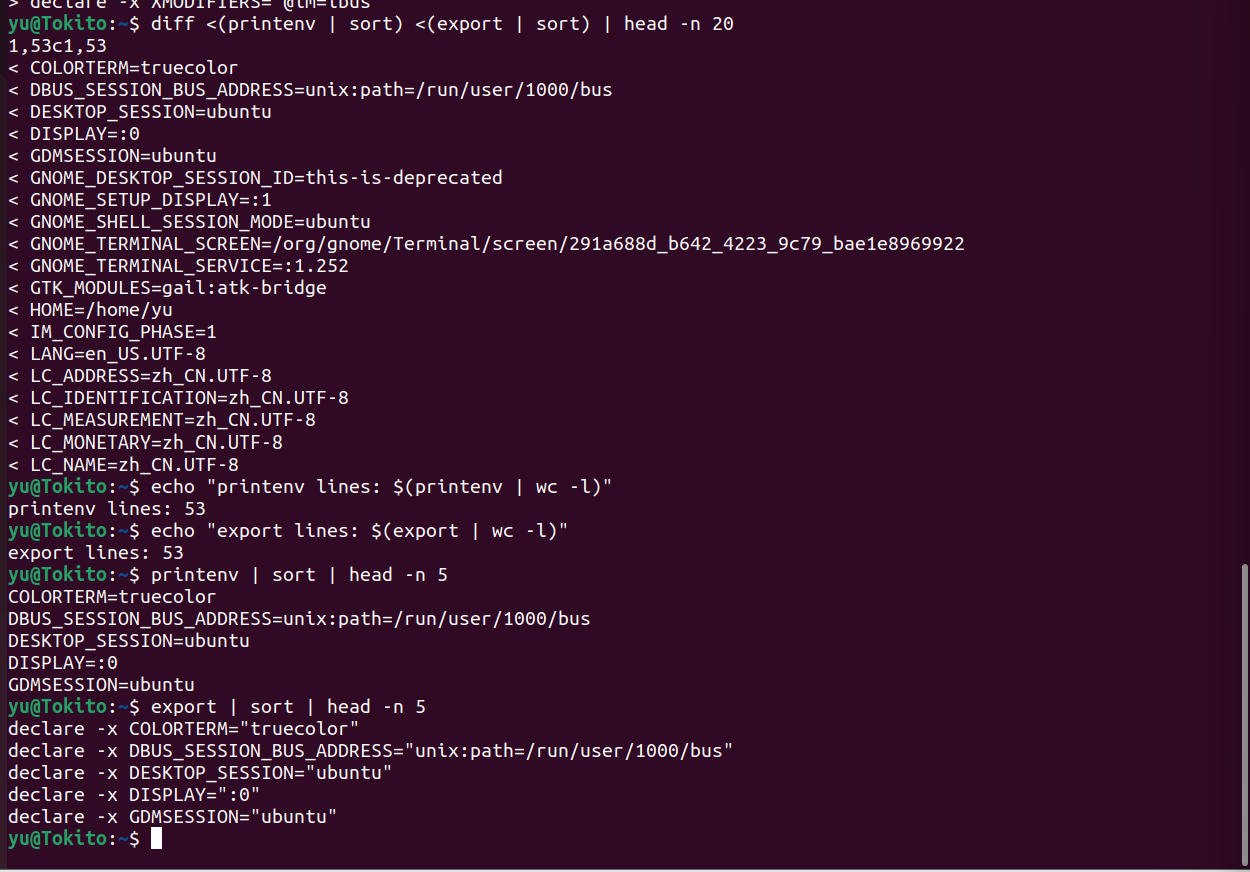
\includegraphics[width=0.92\textwidth]{../screenshots/practice/pra01.png}  
    \caption{练习1：使用 ls -l 查看文件信息}  
    \label{fig:pra01}  
\end{figure}  
  
  
\subsection{练习2：Glob 通配模式}  
  
  
\textbf{做法：}创建多个测试文件，使用不同的通配符进行匹配。  
  
  
\begin{lstlisting}[language=bash]  
touch a.txt b.txt c.txt file1.txt file2.txt file10.txt  
ls *.txt  
ls file?.txt  
ls {a,b,c}.txt  
\end{lstlisting}  
  
  
\textbf{注意：}\texttt{*} 匹配任意长度字符，\texttt{?} 只匹配一个字符，  
所以 \texttt{file?.txt} 不会匹配 \texttt{file10.txt}。  
  
  
\begin{figure}[H]  
    \centering  
    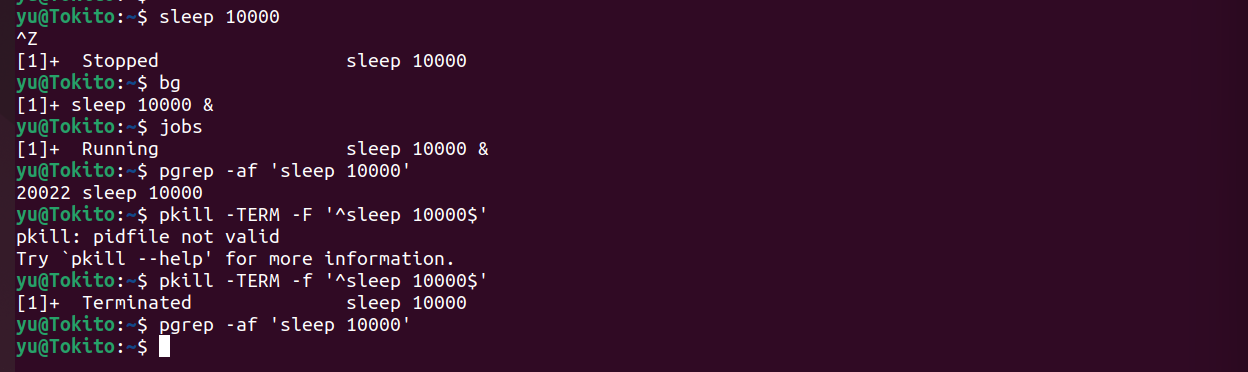
\includegraphics[width=0.92\textwidth]{../screenshots/practice/pra02.png}  
    \caption{练习2：Glob 通配模式}  
    \label{fig:pra02}  
\end{figure}
\subsection{练习3：使用命令连接符控制执行顺序}

\textbf{做法：}使用 \texttt{\&\&}、\texttt{||} 和分号控制多个命令的执行顺序。

\begin{lstlisting}[language=bash]
echo "first command" && echo "second command"
echo "success" || echo "failed"
echo "command A"; echo "command B"
\end{lstlisting}

为了观察命令执行失败时的不同效果，执行：

\begin{lstlisting}[language=bash]
false && echo "this will not be printed"
false || echo "the previous command failed"
false; echo "this command will still be executed"
\end{lstlisting}

\textbf{结果分析：}\texttt{\&\&} 表示当前一个命令执行成功时，
才执行后一个命令；\texttt{||} 表示当前一个命令执行失败时，
才执行后一个命令；分号表示依次执行命令，不关注前一个命令的返回值。
这些连接符可以用于编写 Shell 脚本中的条件控制逻辑。

\begin{figure}[H]
    \centering
    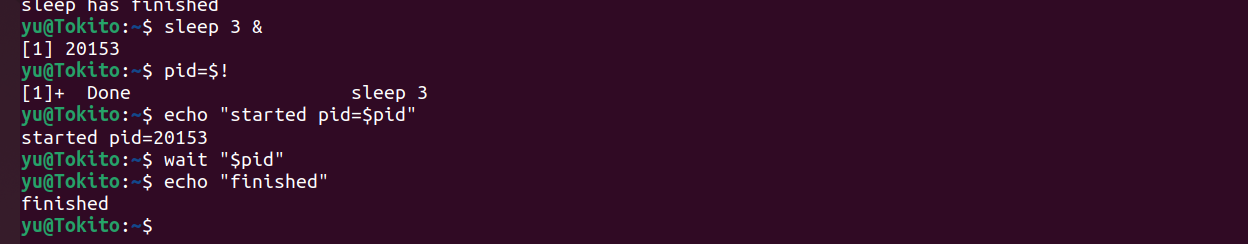
\includegraphics[width=0.92\textwidth]{../screenshots/practice/pra03.png}
    \caption{练习3：使用命令连接符控制执行顺序}
    \label{fig:pra03}
\end{figure}

\subsection{练习4：创建和使用 Shell 别名}

\textbf{做法：}为常用命令设置别名，并验证别名的执行效果。

\begin{lstlisting}[language=bash]
alias gs='git status'
alias ga='git add'
alias ll='ls -alF'
alias py='python3'
\end{lstlisting}

使用以下命令检查别名：

\begin{lstlisting}[language=bash]
alias gs
alias ga
alias ll
alias py
type gs
type py
\end{lstlisting}

分别测试别名：

\begin{lstlisting}[language=bash]
gs
ll
py --version
\end{lstlisting}

\textbf{结果分析：}通过 \texttt{alias} 可以为较长或使用频率较高的
命令设置简短名称。例如，\texttt{gs} 等价于
\texttt{git status}，\texttt{py} 等价于 \texttt{python3}。
使用 \texttt{type} 可以检查当前命令是否为别名。

需要注意，直接在终端中设置的别名只对当前 Shell 会话有效。
若要永久保存，应将配置写入 \texttt{\textasciitilde/.bashrc}，
然后执行 \texttt{source \textasciitilde/.bashrc}。

\begin{figure}[H]
    \centering
    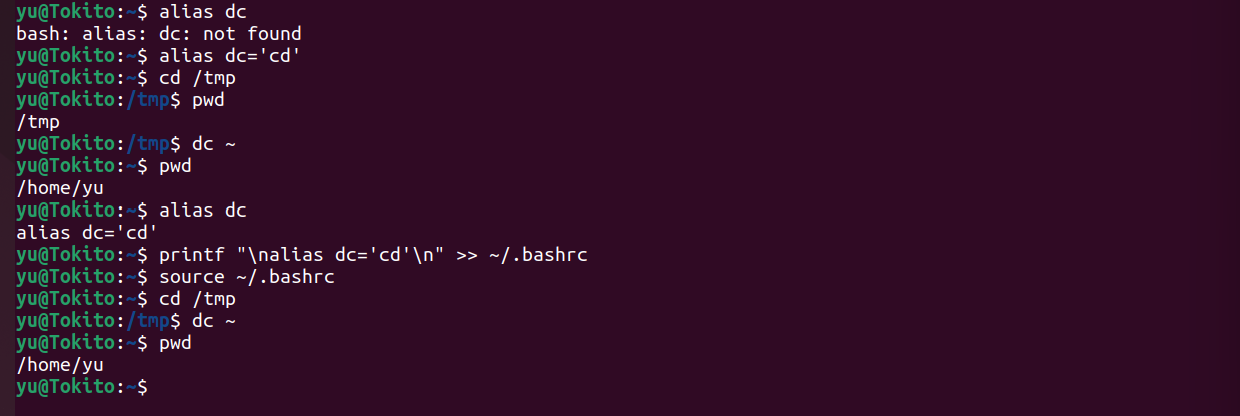
\includegraphics[width=0.92\textwidth]{../screenshots/practice/pra04.png}
    \caption{练习4：创建和验证 Shell 别名}
    \label{fig:pra04}
\end{figure}

\subsection{练习5：统计历史命令的使用频率}

\textbf{做法：}使用 \texttt{history} 获取历史命令，
并结合 \texttt{awk}、\texttt{sort} 和 \texttt{uniq} 统计命令的使用次数。

\begin{lstlisting}[language=bash]
history | awk '{$1=""; print substr($0,2)}' | sort | uniq -c | sort -n | tail -n 10
\end{lstlisting}

为了减少命令中的空格影响，也可以使用下面的方式提取命令名称：

\begin{lstlisting}[language=bash]
history | awk '{$1=""; print $0}' | sed 's/^ *//' | awk '{print $1}' | sort | uniq -c | sort -n | tail -n 10
\end{lstlisting}

根据常用命令配置别名：

\begin{lstlisting}[language=bash]
printf "\nalias gs='git status'\nalias ga='git add'\nalias ll='ls -alF'\nalias py='python3'\n" >> ~/.bashrc
source ~/.bashrc
alias gs
alias ga
alias ll
alias py
\end{lstlisting}

\textbf{结果分析：}\texttt{history} 用于读取历史命令，
\texttt{awk} 用于去除历史编号，\texttt{sort} 用于将相同命令排列在一起，
\texttt{uniq -c} 用于统计重复次数，最后使用
\texttt{sort -n} 和 \texttt{tail -n 10} 得到出现次数较多的命令。

需要注意，使用 \texttt{history} 统计时应避免把统计命令本身
重复计算过多次。配置 alias 后，必须通过
\texttt{source \textasciitilde/.bashrc} 重新加载配置，否则新别名不会在
当前 Shell 中生效。

\begin{figure}[H]
    \centering
    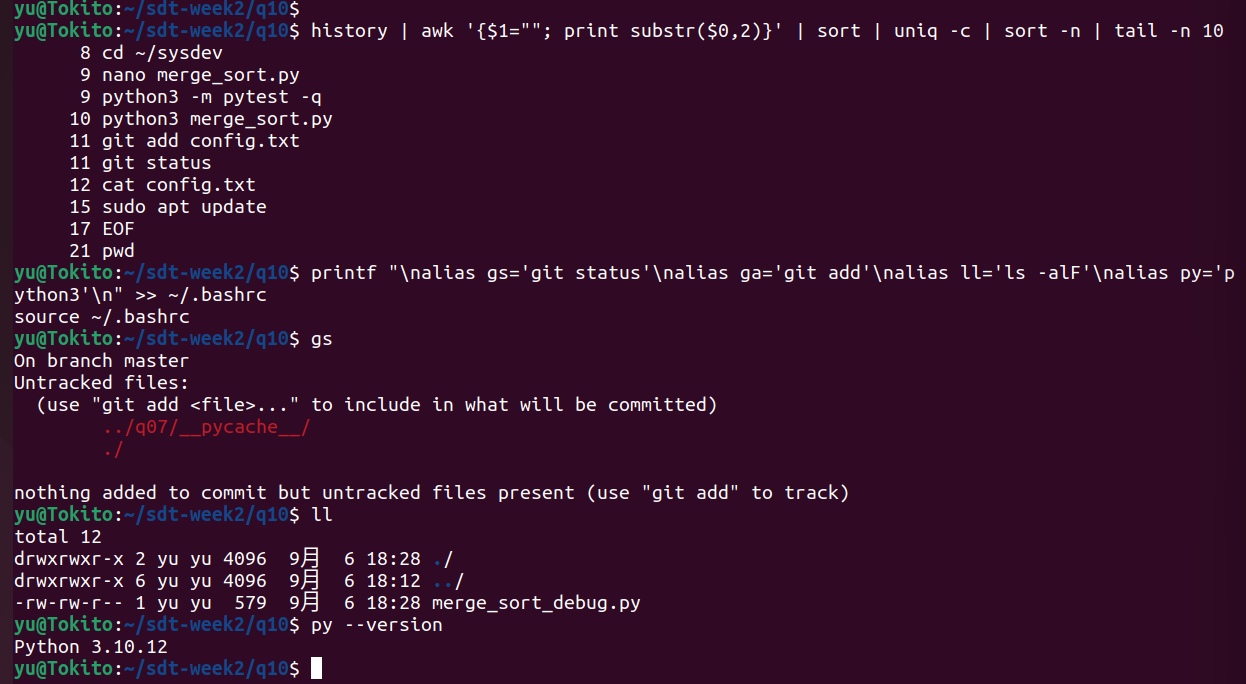
\includegraphics[width=0.92\textwidth]{../screenshots/practice/pra05.png}
    \caption{练习5：统计历史命令并配置常用别名}
    \label{fig:pra05}
\end{figure}

\subsection{练习6：使用 Git 管理配置文件}

\textbf{做法：}创建 dotfiles 目录，将 Bash 配置文件复制到该目录，
并使用 Git 记录配置文件的版本变化。

\begin{lstlisting}[language=bash]
mkdir -p ~/dotfiles
cd ~/dotfiles
cp ~/.bashrc bashrc
git init
git branch -M main
git status
git add bashrc
git commit -m "chore: add bash configuration"
\end{lstlisting}

查看提交记录：

\begin{lstlisting}[language=bash]
git log --oneline --graph --all
git status
\end{lstlisting}

创建 Git 忽略文件，避免提交编辑器产生的临时文件：

\begin{lstlisting}[language=bash]
printf "*.swp\n*~\n" > .gitignore
git add .gitignore
git commit -m "chore: add gitignore"
git status
\end{lstlisting}

\textbf{结果分析：}dotfiles 通常指以点号开头的用户配置文件，
例如 \texttt{.bashrc} 和 \texttt{.gitconfig}。
将配置文件放入 Git 仓库后，可以查看每次修改的提交记录，
也可以在不同计算机之间同步配置。

本实验中每次修改都应单独提交，不能只在实验结束时进行一次全量提交。
提交记录需要保留，并在实验报告中说明。

\begin{figure}[H]
    \centering
    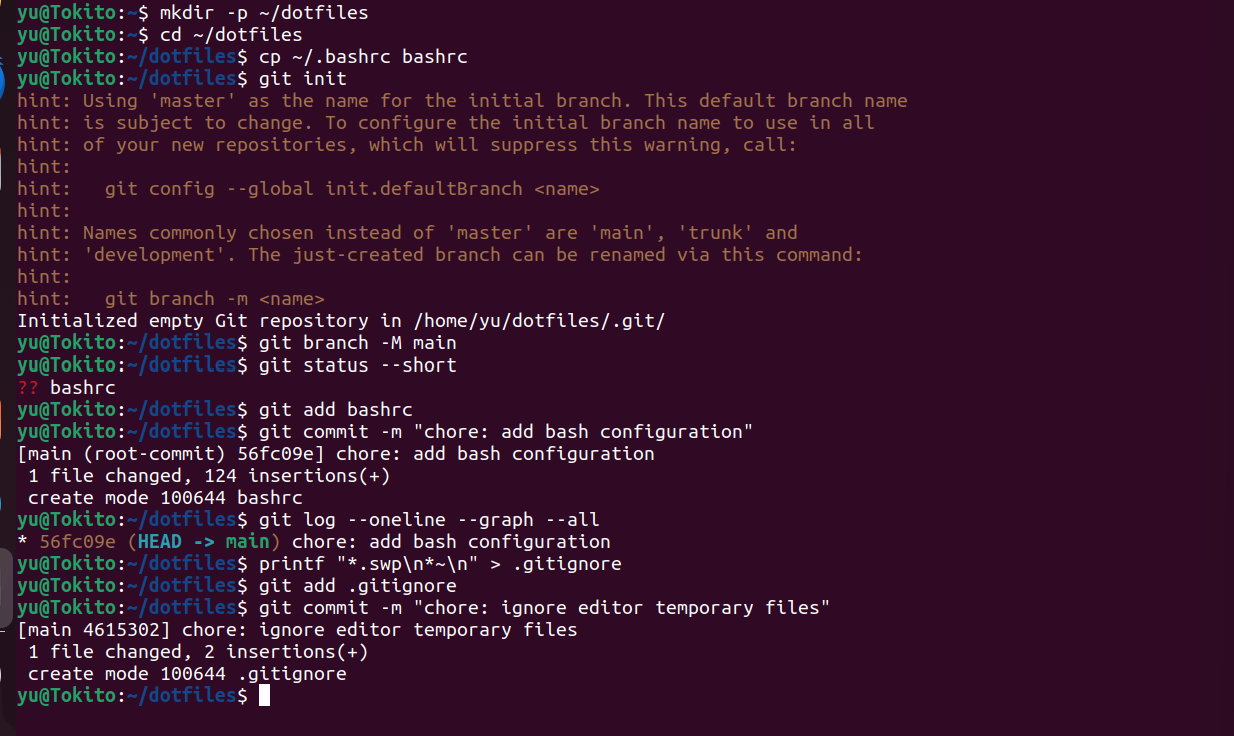
\includegraphics[width=0.92\textwidth]{../screenshots/practice/pra06.png}
    \caption{练习6：使用 Git 管理 Bash 配置文件}
    \label{fig:pra06}
\end{figure}

\subsection{练习7：自定义 Shell 提示符}

\textbf{做法：}通过设置 \texttt{PS1} 修改 Bash 提示符，
使提示符显示用户名、主机名和当前工作目录。

\begin{lstlisting}[language=bash]
export PS1='\u@\h:\w\$ '
echo "$PS1"
\end{lstlisting}

将配置写入 \texttt{\textasciitilde/.bashrc}：

\begin{lstlisting}[language=bash]
printf "\nexport PS1='\\u@\\h:\\w\\$ '\n" >> ~/.bashrc
source ~/.bashrc
\end{lstlisting}

设置带颜色的提示符：

\begin{lstlisting}[language=bash]
export PS1='\[\033[01;32m\]\u@\h\[\033[00m\]:\[\033[01;34m\]\w\[\033[00m\]\$ '
\end{lstlisting}

如果要永久保存带颜色的提示符，可以编辑配置文件：

\begin{lstlisting}[language=bash]
nano ~/.bashrc
\end{lstlisting}

在文件末尾加入：

\begin{lstlisting}[language=bash]
export PS1='\[\033[01;32m\]\u@\h\[\033[00m\]:\[\033[01;34m\]\w\[\033[00m\]\$ '
\end{lstlisting}

保存后重新加载：

\begin{lstlisting}[language=bash]
source ~/.bashrc
\end{lstlisting}

\textbf{结果分析：}\texttt{PS1} 是 Bash 的一级提示符变量。
其中，\texttt{\textbackslash u} 表示用户名，
\texttt{\textbackslash h} 表示主机名，
\texttt{\textbackslash w} 表示当前工作目录。
颜色代码中的 \texttt{01;32m} 表示绿色，
\texttt{01;34m} 表示蓝色，\texttt{00m} 用于恢复默认颜色。

在使用 \texttt{printf} 写入配置文件时，必须对反斜杠进行正确转义，
否则 \texttt{\textbackslash u} 可能被 \texttt{printf} 误认为 Unicode
转义符，从而出现
\texttt{printf: missing unicode digit for \textbackslash u} 错误。

\begin{figure}[H]
    \centering
    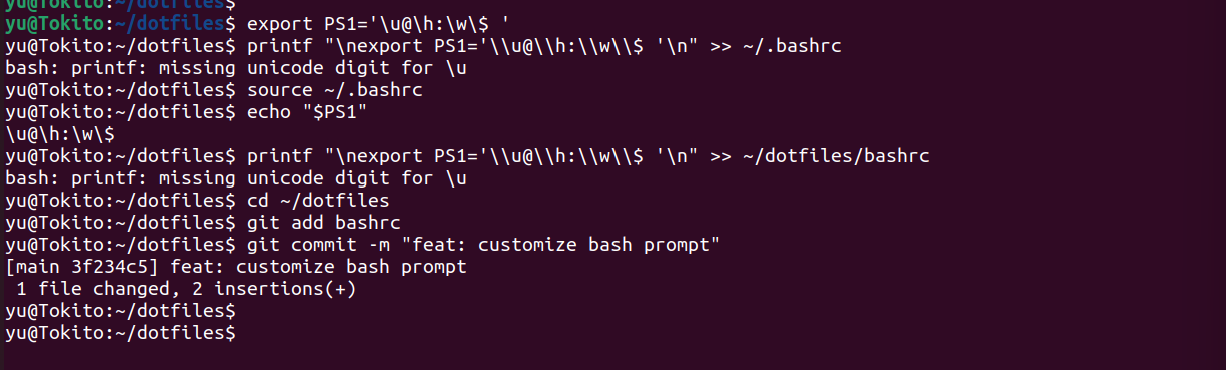
\includegraphics[width=0.92\textwidth]{../screenshots/practice/pra07.png}
    \caption{练习7：自定义带颜色的 Shell 提示符}
    \label{fig:pra07}
\end{figure}

\subsection{练习8：编写 dotfiles 自动安装脚本}

\textbf{做法：}在 \texttt{dotfiles} 目录中编写安装脚本，
使用符号链接部署 Bash 配置文件。

\begin{lstlisting}[language=bash]
cd ~/dotfiles
nano install.sh
\end{lstlisting}

脚本内容如下：

\begin{lstlisting}[language=bash]
#!/usr/bin/env bash
set -e

DOTFILES_DIR="$(cd "$(dirname "${BASH_SOURCE[0]}")" && pwd)"

ln -sfn "$DOTFILES_DIR/bashrc" "$HOME/.bashrc"

echo "dotfiles installed"
echo "Run: source ~/.bashrc"
\end{lstlisting}

为脚本添加执行权限并运行：

\begin{lstlisting}[language=bash]
chmod +x install.sh
./install.sh
ls -l ~/.bashrc
source ~/.bashrc
\end{lstlisting}

检查符号链接的目标：

\begin{lstlisting}[language=bash]
readlink -f ~/.bashrc
\end{lstlisting}

\section{GitHub/Gitee 仓库与提交记录}

代码仓库地址：\url{https://github.com/Tokito-git/sdt-week1-25060012017}

本周实验代码按照 q01、q02、q03、q04 分目录保存。提交过程中采用分步提交方式，分别记录了文件创建、功能实现、错误修复和报告完善等阶段。仓库链接和提交记录截图见图~\ref{fig:git-record}。


\section{实验总结}

本周实验使我认识到，工具链的正确使用不仅是记住命令，还包括对输入、输出、错误状态和历史记录进行验证。Shell 实验中需要特别注意空格路径、隐藏文件、表头和退出码；Git 实验中要根据提交历史理解冲突根因；LaTeX 实验中则需要同时检查源文件、编译引擎和交叉引用。以后进行科研代码或深度学习实验时，熟练使用这些工具能够提高实验复现、问题定位和协作开发的效率。

\section{GitHub/Gitee 仓库与提交记录}

代码仓库地址：\url{https://github.com/Tokito-git/sdt-week1-25060012017}

本周实验代码按照 q01、q02、q03、q04 分目录保存。提交过程中采用分步提交方式，分别记录了文件创建、功能实现、错误修复和报告完善等阶段。仓库链接和提交记录截图见图~\ref{fig:git-record}。

\section{实验总结}

本周实验使我认识到，工具链的正确使用不仅是记住命令，还包括对输入、输出、错误状态和历史记录进行验证。Shell 实验中需要特别注意空格路径、隐藏文件、表头和退出码；Git 实验中要根据提交历史理解冲突根因；LaTeX 实验中则需要同时检查源文件、编译引擎和交叉引用。以后进行科研代码或深度学习实验时，熟练使用这些工具能够提高实验复现、问题定位和协作开发的效率。

\end{document}